\documentclass{beamer}
\usetheme{metropolis}           % Use metropolis theme
\usepackage{tikz-cd}             % Use quiver package for commutative diagrams
\usepackage{tikz}   

\date{\today}
\author{Clément Rouvroy, Grégoire Le Corre, Nathan Boyer}
\institute{Deep Learning Course - M1}
% Define your custom color (e.g., blue)
\definecolor{mBlue}{RGB}{0, 102, 204}

% Override the primary color (orange) with your custom color
\setbeamercolor{frametitle}{bg=mBlue}
\setbeamercolor{progress bar in head/foot}{fg=mBlue}
\setbeamercolor{title separator}{fg=mBlue}
\setbeamercolor{alerted text}{fg=mBlue}
\title{\textcolor{mBlue}{AN} \textcolor{mBlue}{A}rtificial \textcolor{mBlue}{N}eural \textcolor{mBlue}{A}rchitecture \textcolor{mBlue}{S}earch}
\begin{document}
  \maketitle

\section{General Idea}
\begin{frame}{What is a NAS}
    \begin{columns}
        % Left column for the figure
        \column{0.5\textwidth}
        \centering
        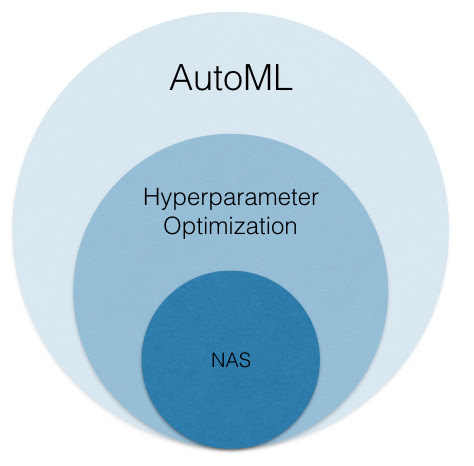
\includegraphics[width=0.9\linewidth]{nas-inclusion.jpg}
        
        % Right column for the centered text
        \column{0.5\textwidth}
        \centering
        \begin{itemize}
            \item[ ]\textcolor{mBlue}{AutoML}: Automating tasks in DL,
            \item[ ] \textcolor{mBlue}{NAS}: Automating model creation and tuning.
        \end{itemize}
        
    \end{columns}

Research started in 2017 with \emph{Neural Architecture Search with Reinforcement Learning} (Google Brain).
\end{frame}

\begin{frame}{Is it working?}

\centering
\begin{figure}
    \centering
    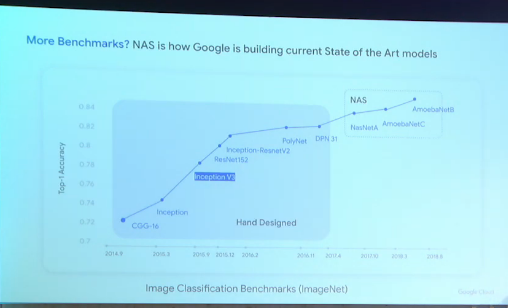
\includegraphics[width=\linewidth]{GOOGLE-2.png}
    \caption{Source: Google Cloud Next 2022}
    \label{fig:enter-label}
\end{figure}


\end{frame}

\section{How it works}

\begin{frame}{Building Blocks}
\begin{itemize}
    \item{\textcolor{mBlue}{Model search spaces} (operations allowed, activation functions, ...)}
    \item{\textcolor{mBlue}{Search strategy} \emph{Estimate} the performance of possible NNs in the space}
    \item{\textcolor{mBlue}{Search algorithm} Receives some metrics about the possible NNs and make a choice. We will optimize it.}
    \item{\textcolor{mBlue}{Model evaluation}: Depends of the usage, some wants a trade-of between speeds and accuracy, some wants full accuracy, ...}
\end{itemize}
\end{frame}

\begin{frame}{Main idea}
\begin{figure}
    \centering
    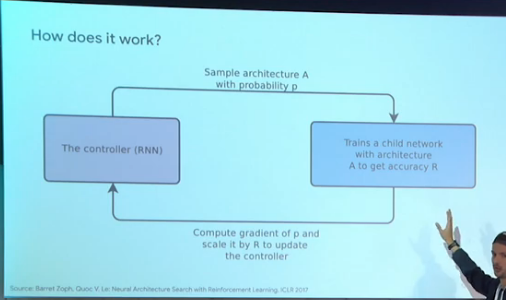
\includegraphics[width=0.6\linewidth]{GOOGLE.png}
    \caption{Workflow illustration (Google Cloud Next 2022)}
    \label{fig:enter-label}
\end{figure}

We are free to define the reward, the optimization policiy and what we allow to compute.

\textcolor{mBlue}{Costs a lot to train at first but then we can generate model with a fewer cost}.
\end{frame}
\end{document}
